% !TeX spellcheck = en_GB
\section{Operational Weather Forecast Model}\label{sec:DIM:MEPS}
MetCoOp Ensemble Prediction System (MEPS) became operational at Met-Norway in November 2016 when the extreme Christmas storm occurred over Norway. Comparing model data with actual observations helps to validate %verify the agreement between 
model predictions. % and ground-based measurements. 
\\
MEPS is used as weather forecast at the Norwegian Meteorological Institute, the Swedish Meteorological and Hydrological Institute (SMHI) and the Finnish Meteorological Institute (FMI), \citep{muller_arome-metcoop:_2017, koltzow_metcoop_2017}.
It replaced Mèteo-France Applications of Research to Operations at MEsoscale (AROME)-MetCoOp, which was operational from March 2014 until November 2016. %, when it was replaced with an ensemble prediction system (EPS) based on AROME-MetCoOp.
%\textcolor{red}{Say more about the model itself! == AROME, Both models are based on...}
Both models are a branch of the Hirlam Aladin Regional Meso-scale Operational NWP In Europe (HARMONIE) AROME model, version 40h1.1. MEPS and AROME-MetCoOp therefore built on the bases of AROME-France a convective-scale model. The physical parametrisations are from the French mesoscale non-hydrostatic atmosphere model (Meso-NH). The model got operational in 2008 and had a horizontal resolution of \SI{2.5}{\km} \citep{seity_arome-france_2010}. 

%Ensemble prediction has the goal to improve the forecast by ensemble averaging, to provide an indication of the reliability of the forecast, and a quantitative basis for probabilistic forecasting \citep{kalnay_atmospheric_2003}. 
\subsection{Ensemble Prediction System}
%%% image Kalnay Fig 6.4.1 %%%%%%%%%%%%%%%%%%%%%%%%%%%%%%%%%%%%%
\begin{figure}[H]
	\centering
    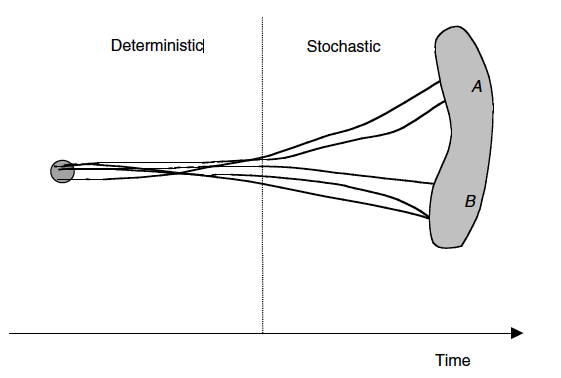
\includegraphics[width=0.49\textwidth]{./fig_MEPS/ensemble}
    \caption{Schematic of ensemble prediction. Circle, representing the uncertainty of the initial conditions. Individual lines, perturbed ensemble member from the initial conditions ending in solution space, grey area \citep{kalnay_atmospheric_2003}.}\label{fig:MEPS:kalnay_ens}
\end{figure}
%%%%%%%%%%%%%%%%%%%%%%%%%%%%%%%%%%%%%%%%%%%%%%%%%%%%%%%%%%%%%%%%%%%%%%%%%%
\noindent
The main difference between AROME-MetCoOP and MEPS is that AROME-MetCoOp only contains a deterministic prediction whereby MEPS has additionally nine individual perturbed ensemble member \citep{metcoop_wiki_description_2017}. 
\\
\Cref{fig:MEPS:kalnay_ens} shows the schematic of an ensemble prediction system (EPS). An ensemble forecasting system requires the definition of the initial amplitude and the horizontal and vertical structure of the perturbation. In general, the initial perturbation is chosen to be close to the observations. The initial condition for the disturbance is within a circle (\Cref{fig:MEPS:kalnay_ens}) of the observation uncertainty. In an ensemble prediction system one of the members is the deterministic forecast (single control forecast) where the other forecast members start from a slight perturbed state of the deterministic forecast. For a short time, should the forecast members be close together, this is a few hours in mesoscale prediction (deterministic in \Cref{fig:MEPS:kalnay_ens}). After a certain period of time, the forecast of the different perturbed members are so large that they have to be considered as stochastic (\Cref{fig:MEPS:kalnay_ens}). 
\\
Important is, that the observations, which are going to be used for the initialisation are within the spread of the individual ensemble member forecasts \citep{kalnay_atmospheric_2003}.

%%%%%%%%%%%%%%%%%%%%%%%%%%%%%%%%%%%%%%%%%%%%%%%%%%%%%%%%%%%%%%%%%%%%%%%%%%
%%%%%%%%%%%%%%%%%%%%%%%%%%%%%%%%%%%%%%%%%%%%%%%%%%%%%%%%%%%%%%%%%%%%%%%%%%
%%%%%%%%% MEPS %%%%%%%%%%%%%%
\subsection{MetCoOP Ensemble Prediction System}\label{sec:AROME}
In principle, MEPS is a short-term weather forecast consisting of ten ensemble members %forecast system 
with \SI{66}{\hour} prediction time and a horizontal resolution of \SI{2.5}{\km} and 65 vertical levels. Hourly \SI{66}{\hour} forecast data is available at Met-Norway for the deterministic and the first perturbed ensemble member. \SI{54}{\hour} forecasts are stored for the three hourly values.
\\
The lower layer, near the ground is approximately \SI{12}{\km} height. With increasing height decreases the vertical resolution of \SIrange{25}{200}{\metre} in the lower \SI{3}{\km}. The model top is at located at approximately \SI{23}{\km}.
The initialisation of each member is performed at \SIlist{00;06;12;18}{\UTC} \citep{metcoop_wiki_description_2017}.
Forecast data saved for the deterministic and first ensemble member have a time resolution of one hour for the \SI{66}{\hour} forecast period. The other eight members have data stored every three hours for up to \SI{48}{\hour} forecast time.
% %\\
%%% image MEPS resolution %%%%%%%%%%%%%%%%%%%%%%%%%%%%%%%%%%%%%
% !TeX spellcheck = en_GB
% \begin{figure}[t]
% 	\centering
%     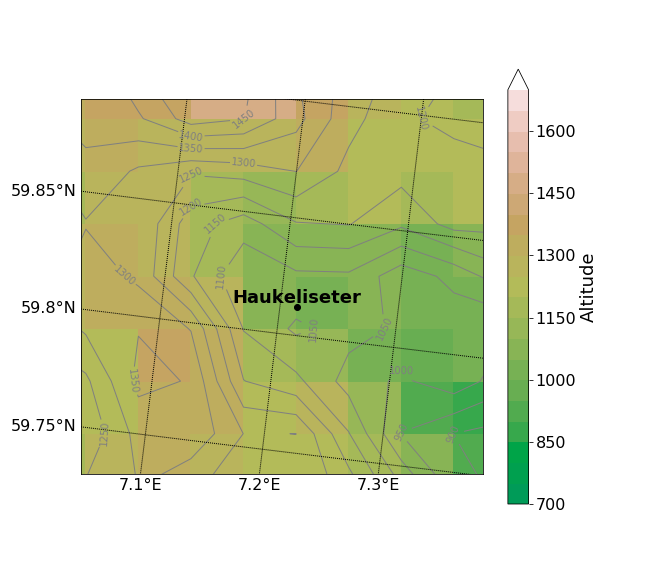
\includegraphics[trim={.3cm 2.2cm 1.8cm 2.4cm},clip,width=\textwidth]{./fig_Norway/MEPS_elevation_Haukeli}
%         \caption{}\label{fig:meps:site}
% \end{figure}

% \begin{wrapfigure}[14]{r}{0.55\textwidth}
% 	\vspace{-\normalbaselineskip}
% 	\centering
% 	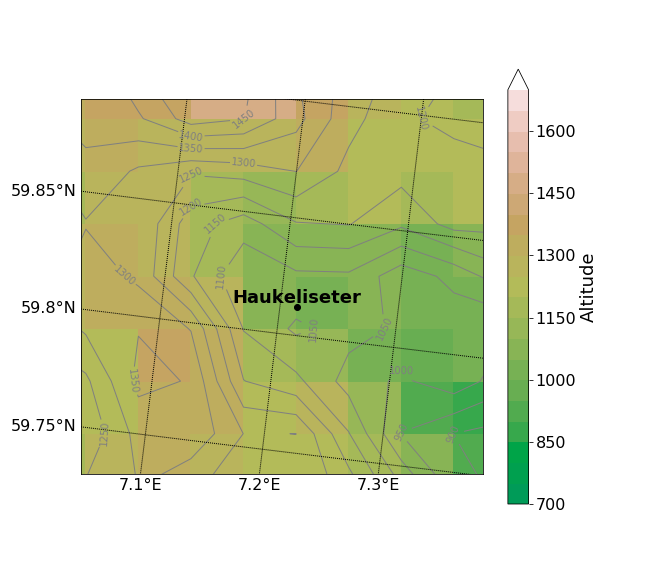
\includegraphics[trim={.3cm 2.2cm 1.8cm 2.4cm},clip,width=0.54\textwidth]{./fig_Norway/MEPS_elevation_Haukeli}
% 	%	\vspace{-10pt}
% 	\caption{Representation of the topography around measurement site Haukeliseter in MEPS. Contours and shading present the elevation of the grid cells.}\label{fig:meps:site}
% 	\vspace{-\normalbaselineskip}
% \end{wrapfigure}

% !TeX spellcheck = en_GB
\begin{figure}[ht!]
	\centering
    \begin{subfigure}[b]{0.53\textwidth}
    	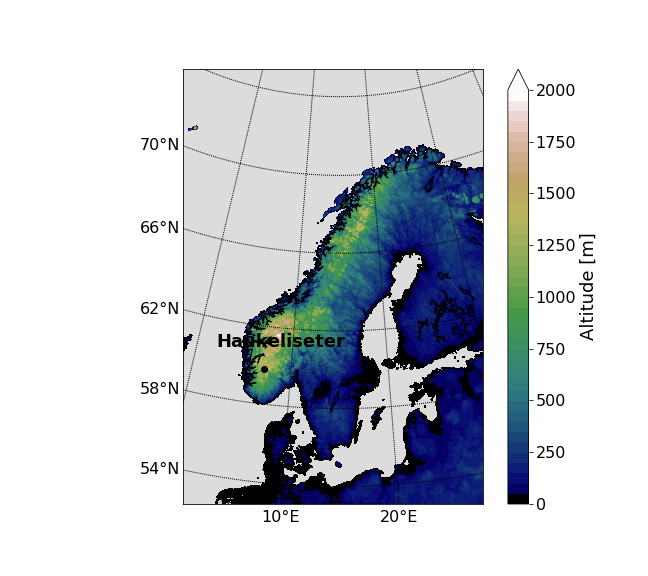
\includegraphics[trim={4.cm 1.8cm 0cm 2.cm},clip,width=1.05\textwidth]{./fig_Norway/Norway_elevation_MEPS}
        \caption{}\label{fig:meps:Norway}
    \end{subfigure}
    \begin{subfigure}[b]{0.46\textwidth}
        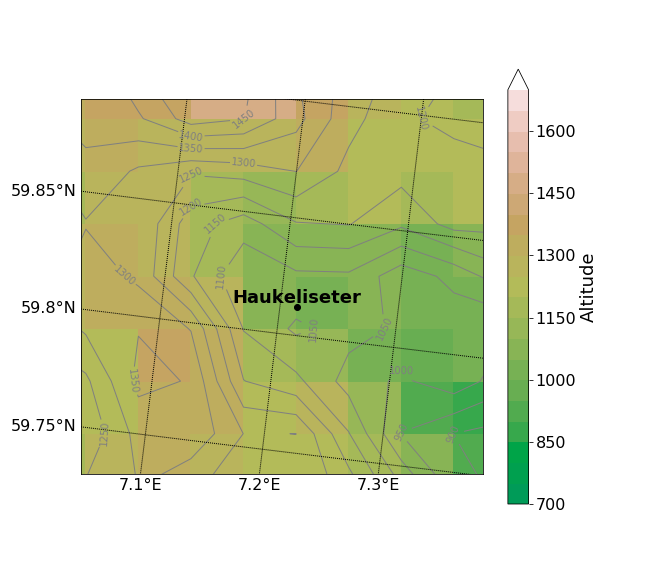
\includegraphics[trim={.3cm 2.2cm 1.8cm 2.4cm},clip,width=\textwidth]{./fig_Norway/MEPS_elevation_Haukeli}
        \caption{}\label{fig:meps:site}
      \end{subfigure}
	\caption{\protect\subref{fig:meps:Norway}: Elevation map of MEPS model domain. \protect\subref{fig:meps:site}: Representation of the topography around the measurement site Haukeliseter in MEPS. Contours and shading present the elevation of the grid cells.}\label{fig:meps_site}
\end{figure} 
%%%%%%%%%%%%%%%%%%%%%%%%%%%%%%%%%%%%%%%%%%%%%%%%%%%%%%%%%%%%%%%%%%%%%%%%%%
\noindent
\Cref{fig:meps:Norway} shows 
the MEPS model domain and its elevation as it was operational for December 2016. It covers Scandinavian countries including open water such as the Atlantic Ocean, the North and the Baltic Seas. 
A representation of the horizontal resolution zoomed for the Haukeliseter site is shown in \Cref{fig:meps:site}. 
%Haukeliseter is surrounded by a complex terrain with mountains up to \SI{1500}{\metre} no the west and the north and the more open terrain to the south-east.
The topographical resolution of MEPS and its influence on local wind and precipitation will be discussed in \Cref{sec:res:oro_infl}.
To compare the measurements from the surface with the MEPS data, the closest model grid point to Haukeliseter, is used (\Cref{fig:meps_site}). The closest grid point to Haukeliseter is \ang{59.80}\,N, \ang{7.22}\,E at \SI{1041}{\metre} above sea level.
\\
The centre of the model is approximately at \ang{63.5}\,N, \ang{15}\,E. 
The horizontal grid points are %projected on a 
Lambert projected to receive the same area size of each grid cell. 
%The outer, parent grid is the ECMWF-IFS model (European Centre for Medium-Range Weather Forecasts Integrated Forecasting System) with a horizontal resolution of \SI{9}{\km} \citep{homleid_verification_2016}. The ECMWF-IFS forecasts are used \SI{6}{\hour} prior to the actual cycle in MEPS.
The regional model MEPS receives initial and boundary conditions from the global ECMWF-IFS (European Centre for Medium-Range Weather Forecasts Integrated Forecasting System) before it can produce its own regional forecasts. In addition, to produce the forecast analysis the background model is initiated for upper-air and surface data assimilation \citep{muller_arome-metcoop:_2017}. 
The horizontal resolution of the parent ECMWF grid is \SI{9}{\km}, has \num{137} model levels, and the model level top is at \SI{80}{\km}. The ECMWF-IFS forecasts are available \SI{5}{\hour} later than the model runs at Met-Norway. MEPS is updated each third hour using obsrvations received in real-time from the global observing system \citep{homleid_verification_2016}.
%used \SI{3}{\hour} prior to the actual cycle in MEPS with.
Since initial conditions such as observations have uncertainties as well as the model has internal variability, it has to reach a background climatology state (spin-up) before the output can be analysed. %has mistrust, and  the own climatology needs to be approached, a model has to stabilize before the simulations can be trusted. 
%The initial conditions such as observations and the model itself have uncertainties. 
\citet{warner_tutorial_1997} states, spin-up time varies depending on the amount and quality of the initial and boundary conditions. If only a few mesoscale initial condition are available then the model should be initialised well before the forecast time. This will allow the model to spin-up mesoscale structures that are responsive to large-scale and local forcing. 
In MEPS, the spin-up time %varies depending on the quality of the initial and boundary conditions, 
can be assumed to be \SI{6}{\hour} for precipitation \citep[personal communication,][]{Priv_Comm_Koltzow}. 
\\
To model the snow in AROME-MetCoOp an one-layer atmosphere model scheme is implemented. The representation is covered by an adjustment of the three-class ice parametrization (ICE3) scheme (\Cref{sec:AROME:adjustment}). 
This includes three variables such as: snow water equivalent (SWE), snow density, and snow albedo \citep{muller_arome-metcoop:_2017}.
How liquid-phase processes are separated from slow ice-phase processes are described in \Cref{sec:MesoNH}. 
% \\
% As synoptic observations are included in the model the snow-depth predictions underlay a special performance. Observations of snow-depth are only available at \SIlist{06;18}{\UTC}, therefore the snow analysis is only performed twice daily \citep{muller_arome-metcoop:_2017, homleid_verification_2016}. 
%%%%%%%%%%%%%%%%%%%%%%%%%%%%%%%%%%%%%%%%%%%%%%%%%%%%%%%%%%%%%%%%%%%%%%%%%%

%%%%%%%%%%%%%%%%%%%%%%%%%%%%%%%%%%%%%%%%%%%%%%%%%%%%%%%%%%%%%%%%%%%%%%%%%%
%%%%%%%%% MESONH %%%%%%%%%%%%%%
\subsection{Meso-NH and the ICE3 Scheme} \label{sec:MesoNH}
The physical parametrisation within AROME is based on the French research communities' Meso-NH. The microphysical scheme in the Meso-NH atmospheric simulation system is based on the Kessler scheme for liquid processes whereas the ICE3 parametrisation scheme is for cold processes \citep{meteo_france_meso-nh_2009}. The purpose of the scheme is to model as correctly as possible the ice phase in the atmosphere. The three-class parametrisation scheme is coupled to a Kessler scheme for the warm processes \citep{pinty_mixed-phased_1998}. \cite{mccumber_comparison_1991} concluded from their case study of simulating two different types of tropical convection, that at least three different ice categories are necessary to cover most precipitation but that applications might be case specific. 
According to the \cite{meteo_france_meso-nh_2009} documentation, the ice phase microphysical scheme includes: 
\begin{itemize}
	\item [$\mathbf{i}$:] pristine ice phase  
	\item [$\mathbf{s}$:] snowflake type from lightly rimed large ice crystals or dry clusters, and
	\item [$\mathbf{g}$:] heavily rimed crystals, such as graupel, frozen drops or hail.
\end{itemize}
% %%% table ice parameters %%%%%%%%%%%%%%%%%%%%%%%%%%%%%%%%%%%%%
% % % !TeX spellcheck = en_GB
\begin{table}[h]
	\begin{center}
		\caption{Characterization parameters from primary ice (r$_i$), snowflakes (r$_s$) and rimed crystals (r$_g$). Values are based on the references in \cite{meteo_france_meso-nh_2009} and in \cite{pinty_mixed-phased_1998}. }\label{tab:ice_parameter}
		\begin{tabular}{l|c|c|c}
			\hline \hline
			& \textbf{r$_i$}& \textbf{r$_s$}& \textbf{r$_g$} \\ \hline\hline
			$\alpha$, $\nu$ & \num{3.3}		& \num{1.1}			& \num{1.1} \\ \hline
			$a$				& \num{0.82}	& \num{0.02}		& \num{196} \\ 
			$b$				& \num{2.5}		& \num{1.9}			& \num{2.8} \\ \hline
			$c$				& \num{800}		& \num{5.1}			& \num{124} \\ 
			$d$				& \num{1.0}		& \num{0.27}		& \num{0.66} \\ \hline
			$C$				&				& \num{5}			& \num{5e5} \\
			$x$				&				& \num{1}			& \num{-0.5} \\
			\hline \hline
		\end{tabular}
	\end{center}
\end{table}
% %%%%%%%%%%%%%%%%%%%%%%%%%%%%%%%%%%%%%%%%%%%%%%%%%%%%%%%%%%%%%%%%%%%%%%%%%%
Within the ICE3 scheme no distinction between hail and graupel exists and therefore the physical discrimination is in the growth mode of graupel and hail is neglected. \\
To achieve snow water content within MEPS the number intercept parameter ($N_0$, [\SI{}{\metre^{-3}\per\mm}]), slope parameter of exponential size distribution ($\lambda$, [\SI{}{\per\metre}]), mass diameter ($D$, [\SI{}{\mm}]) and  the particle size distribution [\SI{}{\metre^{-3}\per\mm}] of pristine ice ($n_\mathbf{i}$), snowflakes ($n_\mathbf{s}$), and rimed crystals ($n_\mathbf{g}$)  has to be determined. 
According to \cite{caniaux_numerical_1994}, the particle size distribution in the ICE3 scheme follows the Marshall-Palmer distribution (\Cref{eq:num_dens}). The goal in ICE3 is to use a varying intercept parameter dependent on the ice category. The study of \citet{caniaux_numerical_1994} has shown that $N_0$ can be parametrised with:
\begin{align}
	N_0 & = C \lambda^x  \label{eq:model_N0}
	\\
	\log_{10}C & = -3.55x + 3.89  \nonumber
\end{align}
where $C$ and $x$ are constants depending on the ice category %and represent the relation between each other in 
(\Cref{eq:model_N0}). 
\\
The ice water content for primary ice, snowflakes, and rimed crystals is then assumed to be similar to \Cref{eq:SWC}, but the integration limits range from zero to infinity and mass (($m$, [\SI{}{\kg}])), and particle size distribution ($n(D)$) are dependent on the diameter of the hydrometeor particle. The mass of a single particle and PSD (\Cref{eq:mass_diameter,eq:PSD_MEPS}) are represented depending on the ice category (\Cref{tab:ice_parameter})
\begin{align}
	m(D) & = aD^b 	\label{eq:mass_diameter} \\
	n(D) & = N_0 g(D)	\label{eq:PSD_MEPS}
\end{align}
$a$, $b$ are the characterisations of the parameters according to their type (\Cref{tab:ice_parameter}) and $g(D)$ the generalised Gamma function: 
\begin{align}
	g(D) = \frac{\alpha}{\Gamma(\nu)} \lambda^{\alpha \nu} D^{\alpha \nu -1} \exp\left( -(\lambda D)^\alpha \right)
\end{align}
with $\alpha$, $\nu$ the shape and tail dispersion parameters and $\Gamma(\nu)$ the gamma function. 
\\
After following the above equations including \Cref{eq:SWC} the exponential slope parameter of pristine ice, snow, and rimed crystals, $\lambda$ can be generated with $G(b)$, the gamma function:
\begin{align}
	\lambda & = \left( \frac{\text{SWC}}{aCG(b)}\right)^{\frac{1}{x-b}}
\end{align}
\\
For all hydrometeors the terminal fall velocity based on the diameter, $D$ is assumed.
\begin{align}
	V(D) = c D^d \left(\frac{\rho_{00}}{\rho_{dref}}\right)^0.4 . \label{eq:fall_velo_MEPS}
\end{align}
In \Cref{eq:fall_velo_MEPS} the last factor is the \citet{foote_terminal_1969} correction of the air density and $\rho_{00}$ being the air density at the reference pressure level $P_{00}$.
%
%%% table ice parameters %%%%%%%%%%%%%%%%%%%%%%%%%%%%%%%%%%%%%
% % !TeX spellcheck = en_GB
\begin{table}[h]
	\begin{center}
		\caption{Characterization parameters from primary ice (r$_i$), snowflakes (r$_s$) and rimed crystals (r$_g$). Values are based on the references in \cite{meteo_france_meso-nh_2009} and in \cite{pinty_mixed-phased_1998}. }\label{tab:ice_parameter}
		\begin{tabular}{l|c|c|c}
			\hline \hline
			& \textbf{r$_i$}& \textbf{r$_s$}& \textbf{r$_g$} \\ \hline\hline
			$\alpha$, $\nu$ & \num{3.3}		& \num{1.1}			& \num{1.1} \\ \hline
			$a$				& \num{0.82}	& \num{0.02}		& \num{196} \\ 
			$b$				& \num{2.5}		& \num{1.9}			& \num{2.8} \\ \hline
			$c$				& \num{800}		& \num{5.1}			& \num{124} \\ 
			$d$				& \num{1.0}		& \num{0.27}		& \num{0.66} \\ \hline
			$C$				&				& \num{5}			& \num{5e5} \\
			$x$				&				& \num{1}			& \num{-0.5} \\
			\hline \hline
		\end{tabular}
	\end{center}
\end{table}
%%%%%%%%%%%%%%%%%%%%%%%%%%%%%%%%%%%%%%%%%%%%%%%%%%%%%%%%%%%%%%%%%%%%%%%%%%
%
%%% image ICE3 scheme  %%%%%%%%%%%%%%%%%%%%%%%%%%%%%%%%%%%%%
% !TeX spellcheck = en_GB
\begin{figure}[h]
	\centering
	%    \begin{subfigure}[b]{\textwidth}
	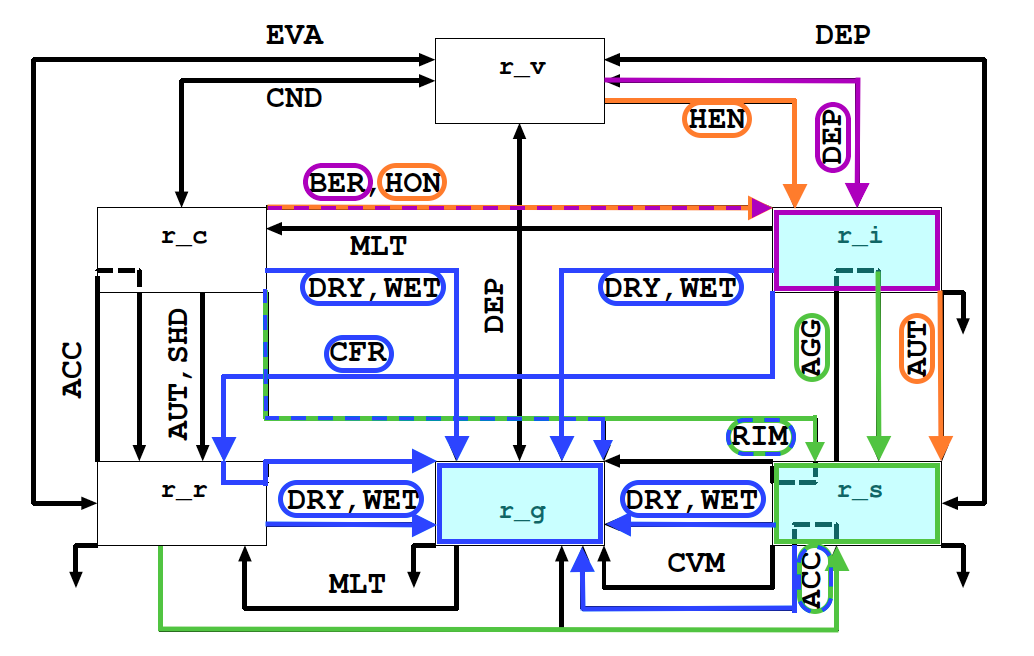
\includegraphics[width=\textwidth]{./fig_MEPS/ICE3_scheme_copy}
	%	\end{subfigure}
	\caption{Microphysical processes for mixed phase clouds in the ICE3 scheme adapted from \cite{meteo_france_meso-nh_2009}. In orange the initiation processes for primary ice r$_i$ and snowflakes r$_s$. The growing processes of r$_i$ is shown in purple and for r$_s$ in green. Graupel particles, r$_g$, grow from existent particles and the processes are shown in blue. }\label{fig:ICE3_scheme}
\end{figure}
%%%%%%%%%%%%%%%%%%%%%%%%%%%%%%%%%%%%%%%%%%%%%%%%%%%%%%%%%%%%%%%%%%%%%%%%%%
\noindent
\Cref{fig:ICE3_scheme} shows the summary of the microphysical processes for mixed phase clouds. The study focuses mostly on solid precipitation particles and therefore only the initiation and growth of pristine ice crystals $\mathbf{i}$, snowflakes $\mathbf{s}$, and rimed crystals $\mathbf{g}$ is presented. 
\\
Following \cite{pinty_mixed-phased_1998} and \Cref{fig:ICE3_scheme} it can be seen how AROME calculates ice growth. %
\begin{itemize}
\item The ICE3 scheme starts with \textit{cold} - 'slow' processes for ice processes (right side in \Cref{fig:ICE3_scheme}) 
	\begin{itemize}
	\item homogeneous (HON) and heteorogeneous (HEN) nucleation
    \item vapour deposition of snow and graupel particles (DEP)
    \item aggregation (AGG) and auto conversion (AUT)
	\end{itemize}
\item The second step is to initiate the \textit{warm} processes (left side in \Cref{fig:ICE3_scheme})
\item Then including the 
	\begin{itemize}
	\item aggregation and conversion-melting (CVM) for snowflakes and 
    \item contact freezing of raindrops (CFR)
	\end{itemize}
\item Followed by AGG and melting for graupel (MLT)
\item And the melting from pristine ice and the Wegener-Bergeron-Findeisen (BER) effect
\item finally integrate the sedimentation terms
\end{itemize}

%\cite{meteo_france_meso-nh_2009} documentation suggests starting the microphysics in the ICE3 scheme with 'slow' processes such as homogeneous and heterogeneous nucleation (HON, HEN), vapour deposition of snow and graupel particles (DEP), aggregation (AGG) and auto conversion (AUT), for ice processes right side in \Cref{fig:ICE3_scheme}. The second step is to initiate the warm processes left side in \Cref{fig:ICE3_scheme}. Then include the aggregation and conversion-melting (CVM) for snowflakes and contact freezing of raindrops (CFR). Add AGG and melting for graupel (MLT), and then the melting from pristine ice  and the Wegener-Bergeron-Findeisen (BER) effect and lastly the sedimentation terms.  \\

% are the primary ice crystals activated by either heterogeneous nucleation (HEN), when some ice nuclei are present or by homogeneous nucleation (HON), when the atmospheric temperature is below \SI{-35}{\celsius}. The growing process for these particles can be the Bergeron-Findeisen process (BER) or deposition of water vapour (DEP). \\
% Snow particles are initiated by auto conversion (AUT) of r$_i$ and grow by the riming of cloud droplets (RIM) or rain droplets (ACC), and by collection of small pristine crystals (AGG), indicated by the green lines in \Cref{fig:ICE3_scheme}. \\
% As indicated by the blue lines in \Cref{fig:ICE3_scheme} are graupel an effect of heavy riming and grow in the scheme if the riming aggregates are of larger diameter size than \SI{7}{\mm} \citep{meteo_france_meso-nh_2009}. As indicated can graupel also grow when larger colliding raindrops reshape snowflakes to graupel (ACC). Furthermore, is graupel growth affected by wet or dry (WET, DRY) accretion, when the surface temperature of graupel is larger than the environmental temperature. DRY graupel expansion happens as long as the surface temperature is less that the surrounding temperature, then collected drops will freeze. WET graupel growth appears, when a liquid film is on the surface of the graupel particle (surface temperature larger than surrounding) then the liquid condensate is shed away, and hail will be formed. In ICE3 is hail not specifically included it is mixed in to the graupel category and therefore a distinction between the two categories cannot be made. 

%
%\newpage
\subsection{AROME-MetCoOp Adjustment}\label{sec:AROME:adjustment}
% refinement for AROME 
Since the ICE3 scheme showed some weaknesses in AROME-MetCoOp for the boreal winter month, \cite{muller_arome-metcoop:_2017} introduced some modifications. 
During cold conditions (\SI{2}{\metre} temperature between \SIlist{-5;-10}{\celsius}) the ICE3-scheme followed too low \SI{2}{\metre} temperature in AROME-MetCoOp. Furthermore, too much ice fog or low clouds were simulated for \SI{2}{\metre} temperature $\le$ \SI{-15}{\celsius} all year long. After implementing the modifications such as separating fast liquid-phase processes from the slower ice-processes, as well as reducing sublimation speed of ice particles. Also, taking into account the difference of optical thickness between ice-phase clouds and water-, mixed-clouds reduced the negative \SI{2}{\metre} bias \citep{muller_arome-metcoop:_2017} %the two meter temperature bias was reduced as well as an improvement of low-level clouds was shown. 
A negative aspect of these adjustments was that the occurrence of fog increased.%, by an error in the surface scheme.

% %%%%%%%%%%%%%%%%%%%%%%%%%%%%%%%%%%%%%%%%%%%%%%%%%%%%%%%%%%%%%%%%%%%%%%%%%%
% %%%%%%%%%%%%%%%%%%%%%%%%%%%%%%%%%%%%%%%%%%%%%%%%%%%%%%%%%%%%%%%%%%%%%%%%%%
% %%%%%%%%% SURFEX %%%%%%%%%%%%%%
% \section{SURFEX}
% \cite{masson_surfexv7.2_2013} \\
% SURFEX stands for 'surface externalisée' and is introduced into NWP models to ensure the consistent treatment of surface processes. It simulates the exchange of energy between four surface types and the atmosphere \citep{homleid_verification_2016}.

%%%%%%%%%%%%%%%%%%%%%%%%%%%%%%%%%%%%%%%%%%%%%%%%%%%%%%%%%%%%%%%%%%%%%%%%%%
%%%%%%%%%%%%%%%%%%%%%%%%%%%%%%%%%%%%%%%%%%%%%%%%%%%%%%%%%%%%%%%%%%%%%%%%%%












